\documentclass{article}

\usepackage{fullpage}
\usepackage{graphicx}
\usepackage{grffile}
\usepackage{amsmath}

\begin{document}

\title{Time Step Size Dependence of the Unsplitting Implicit Midpoint Predictor-Corrector Scheme: 1D, 2D, and 3D Cases\footnote{For the actual run script, inputs file, and post-pocessing scripts, see \texttt{exec/reactDiff/test/misc/Schlogl\_hist\_1d}, \texttt{Schlogl\_hist\_2d}, and \texttt{Schlogl\_hist\_3d}.}}
\author{}
\date{}
\maketitle

\section{Overview}
From the structure factor analysis of the linearized reaction-diffusion SPDE, it has been shown that the unsplitting implicit midpoint predictor-corrector scheme exhibits more favorable behaviors than other schemes.
On the other hand, from the numerical simulation of the one-dimensional Schlogl model in equilibrium, several averaging methods and multiplicative noise expressions for the stochastic diffusive flux have been tested, and it has been shown that the arithmetic-mean averaging type and $n^*=\left(2 n^\mathrm{pred}-n^\mathrm{old}\right)^+$ for the term $\sqrt{2\chi n^*}$ in the corrector stage work better than other options.

In this report, for the implicit midpoint scheme with these options, we investigate the dependence of the scheme on time step size $\Delta t$.
In other words, we observe how the scheme behaves as $\Delta t$ is increased.
One interesting question is whether the time step producing reliable results is dependent on the dimensionality of the system.
To this end, we introduce two \textit{quantitative} measures that indicate how reliabe the scheme is: the probability of negative cell number density and the Kullback--Leibler (KL) divergence.
The latter measures how the histogram obtained from the scheme is different from the Poisson statistics, which is defined as follows:
\begin{equation}
\label{KLdiv}
D_\mathrm{KL}(P||Q)=\sum_i P_i \log \frac{P_i}{Q_i},
\end{equation}
where $P$ and $Q$ denote the distributions of cell number density based on the Poisson statistics and the histogram, respectively, and the sum is over all physically admissible values (i.e., $i/\Delta V$, $i=0,1,\dots$).
Note that these two measures are completely computable from the cell number density distribution $\rho(n)$.

\section{Computational Details}

\subsection{System and Numerical Scheme}

\begin{itemize}

\item Physical parameters
\begin{itemize}
\item Diffusion: diffusion coefficient $\chi=1$
\item Reaction: Schlogl model in equilibrium with $k_1=k_2=k_3=k_4=0.1$ ($n_\mathrm{eq}=1$)
\item Average number of particles per cell: $N_\mathrm{av}=10$
\end{itemize}

\item Spatial discretization
\begin{itemize}
\item 1D: 64 cells ($\Delta x=1$)
\item 2D: $64\times64$ cells ($\Delta x=\Delta y=1$)
\item 3D: $32\times32\times32$ cells ($\Delta x=\Delta y=\Delta z=1$)
\item Volume adjusting factor (or cross section) $A=10$ is used so that $\Delta V=10$ and $N_\mathrm{av}=n_\mathrm{eq}\Delta V=10$.
\item Periodic boundary conditions
\item \texttt{avg\_type=1}
\end{itemize}

\item Temporal integrator
\begin{itemize}
\item Unsplitting implicit midpoint predictor-corrector scheme
\item \texttt{midpoint\_stoch\_flux\_type=3}
\item Time step size: $\Delta t=0.1$, 0.25, 0.5, 1, and 2
\end{itemize}

\item Dimensionless numbers
\begin{itemize}
\item Diffusion: $\beta=\frac{\chi\Delta t}{\Delta x^2}=\Delta t$
\item Reaction: $\alpha = r\Delta t = 0.2\Delta t$
\item $\beta=5\alpha$
\end{itemize}

\end{itemize}

\subsection{Calculation of Physical Quantities}

The following quantities were calculated from the trajectory data (\texttt{fort.10}) of cell number densities $n_j(k\Delta t_\mathrm{traj})$:
\begin{itemize}
\item Probability of negative density,
\item KL divergence,
\item Mean and variance of cell number density,
\item Histogram of cell number density.
\end{itemize}
The initial trajectory data up to physical time $1000$ were discarded to obtain equilibrium trajectory, and the cell number densities were obtained every physical time $\Delta t_\mathrm{traj}=1$ (except for $\Delta t=\Delta t_\mathrm{traj}=2$).
For 1D, $16$ runs with different random seeds were performed and $10^4$ configurations were collected from each run.
For 2D and 3D, single runs were performed and 5000 and 1000 configurations were collected, respectively.
Note that a smaller number of configurations were obtained for higher dimensions since there are more cell number density data in each configuration.\footnote{This is valid for any physical quantity that can be completely determined by the distribution of cell number density $\rho(n)$. However, if a quantity depends on the correlation between cells (e.g., the structure factor $S(k)$), this is no more valid.}
Also, note that when the KL divergence was calculated from Eq.~\eqref{KLdiv}, the sum was calculated only for $Q_i>0$.\footnote{In principle, the KL divergence is defined only if $Q_i=0$ implies $P_i=0$, which cannot hold for the Poisson statistics $P$ and numerically obtained histogram $Q$.}

\section{Results}

In Figures~\ref{fig_negdens} and \ref{fig_KLdiv}, the proability of negative density and the KL divergence are shown.
The main observation is that for higher dimensions the deviations of numerical results from theoretical predictions based on the Poisson statistics become larger.
In other words, the time step size giving reliable results depends on the dimensionality of the system.
In the right columns of the figures, the physical quantities are plotted versus the time step size multiplified by the dimensionality of the system.
Although the agreement of curves of 1D, 2D, and 3D cases are not perfect, the time step needed for reliable results seems to be inversely proportional to the dimensionality of the system.

As supplemental data, the mean and variance of cell number density (in Fig.~\ref{fig_meanvar}) and the histogram of cell number density (in Figs.~\ref{fig_1d_DIFF_hist}--\ref{fig_3d_REACT_hist}) are also shown in this report.

\begin{figure}
\begin{center}
\framebox[1.2\width]{Probability of Negative Density}\\
\vspace{5mm}
(a) Diffusion-Only
\vspace{-5mm}
\end{center}
\includegraphics[angle=270,width=\linewidth]{fig1/negdens_diff.eps}
\begin{center}
(b) Reaction + Diffusion
\vspace{-5mm}
\end{center}
\includegraphics[angle=270,width=\linewidth]{fig1/negdens_react.eps}
\caption{\label{fig_negdens}}
\end{figure}

\begin{figure}
\begin{center}
\framebox[1.2\width]{KL Divergence}\\
\vspace{5mm}
(a) Diffusion-Only
\vspace{-5mm}
\end{center}
\includegraphics[angle=270,width=\linewidth]{fig1/KLdiv_diff.eps}
\begin{center}
(b) Reaction + Diffusion
\vspace{-5mm}
\end{center}
\includegraphics[angle=270,width=\linewidth]{fig1/KLdiv_react.eps}
\caption{\label{fig_KLdiv}}
\end{figure}

\begin{figure}
\begin{center}
\framebox[1.2\width]{Mean and Variance of Cell Number Density}\\
\vspace{5mm}
(a) Variance, Diffusion-Only
\vspace{-5mm}
\end{center}
\includegraphics[angle=270,width=\linewidth]{fig1/var_diff.eps}
\begin{center}
(b) Variance, Reaction + Diffusion
\vspace{-5mm}
\end{center}
\includegraphics[angle=270,width=\linewidth]{fig1/var_react.eps}
\begin{center}
(c) Mean, Reaction + Diffusion
\vspace{-5mm}
\end{center}
\includegraphics[angle=270,width=\linewidth]{fig1/mean_react.eps}
\caption{\label{fig_meanvar}}
\end{figure}

\begin{figure}
\begin{center}
\framebox[1.2\width]{1D, Diffusion-Only}
\end{center}
\begin{tabular}{cc}
(a) $\Delta t=0.1$ & (b) $\Delta t=0.25$ \\
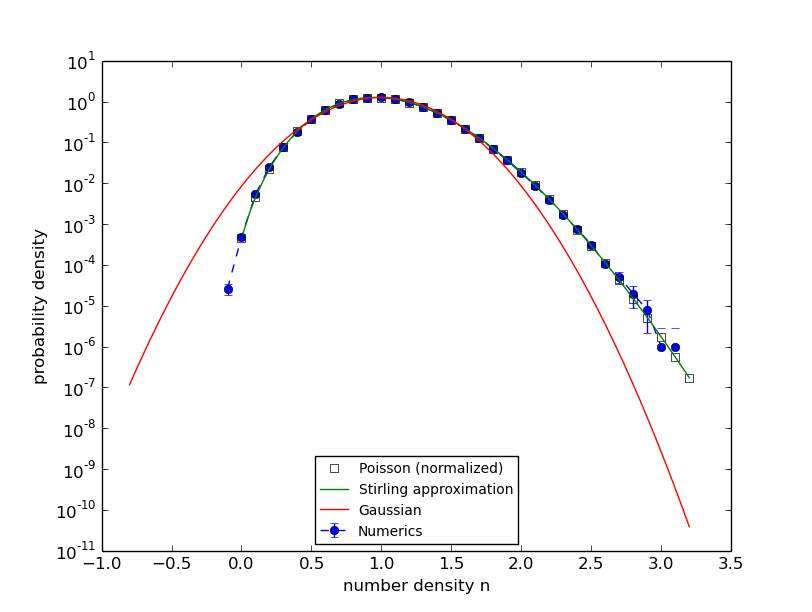
\includegraphics[width=0.5\linewidth]{fig1/1d_DIFF_dt0.1_hist.png} &
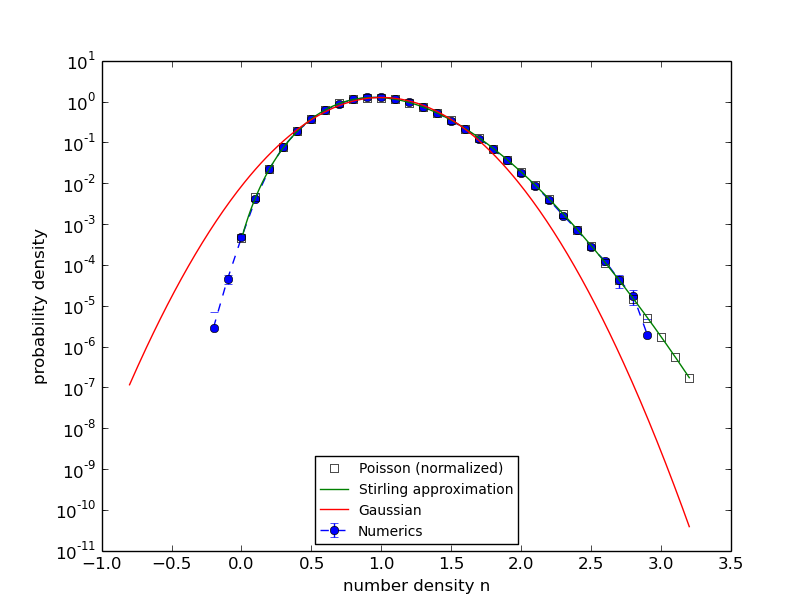
\includegraphics[width=0.5\linewidth]{fig1/1d_DIFF_dt0.25_hist.png} \\
(c) $\Delta t=0.5$ & (d) $\Delta t=1$ \\
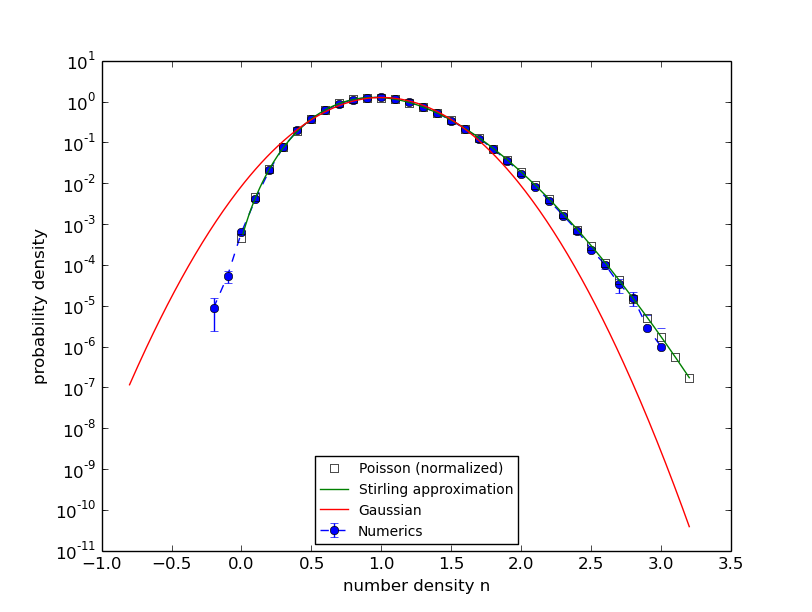
\includegraphics[width=0.5\linewidth]{fig1/1d_DIFF_dt0.5_hist.png} &
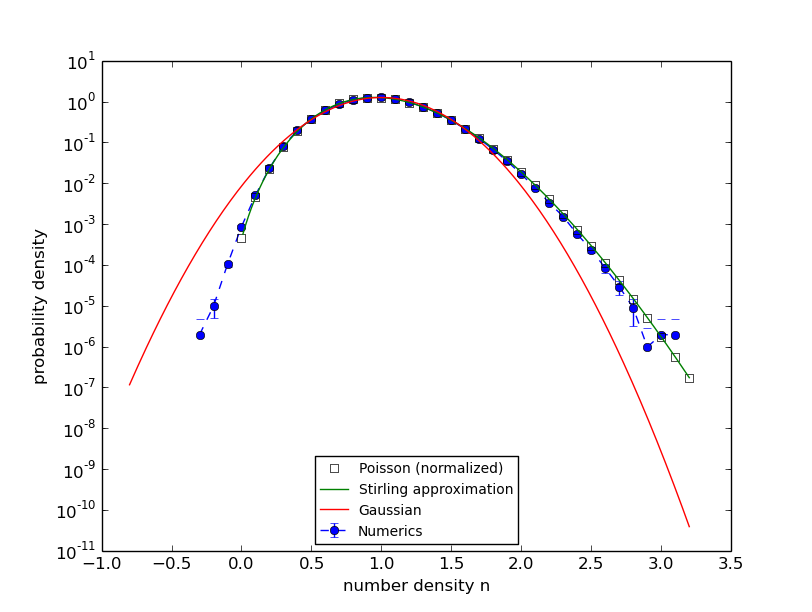
\includegraphics[width=0.5\linewidth]{fig1/1d_DIFF_dt1_hist.png} \\ 
(e) $\Delta t=2$ & \\
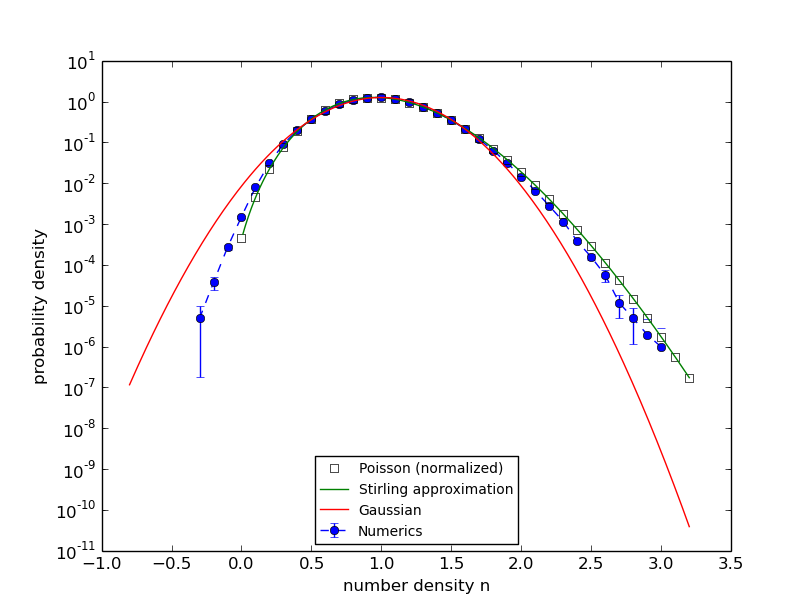
\includegraphics[width=0.5\linewidth]{fig1/1d_DIFF_dt2_hist.png} &
\end{tabular}
\caption{\label{fig_1d_DIFF_hist}}
\end{figure}

\begin{figure}
\begin{center}
\framebox[1.2\width]{1D, Reaction + Diffusion}
\end{center}
\begin{tabular}{cc}
(a) $\Delta t=0.1$ & (b) $\Delta t=0.25$ \\
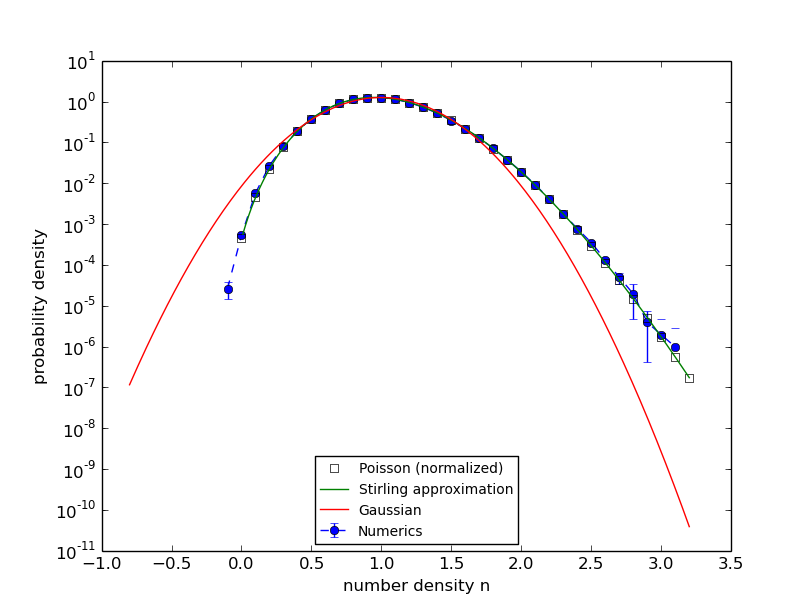
\includegraphics[width=0.5\linewidth]{fig1/1d_REACT_dt0.1_hist.png} &
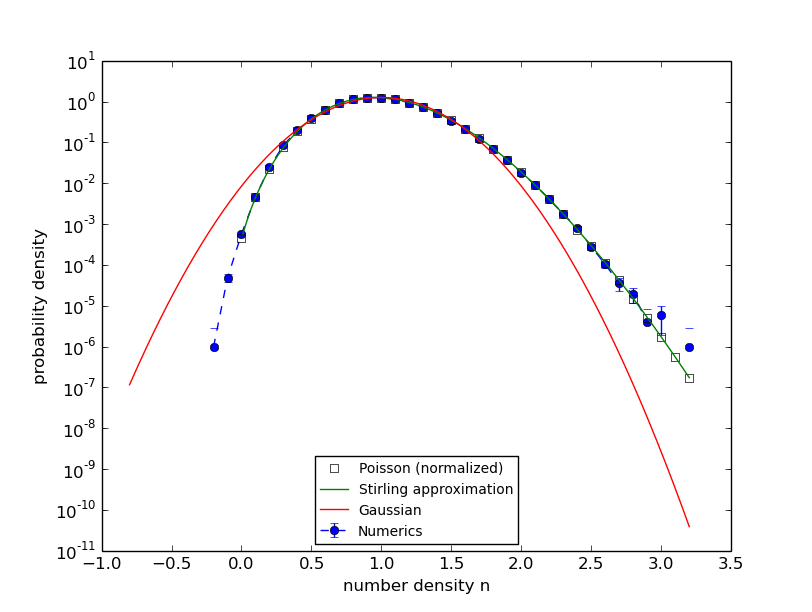
\includegraphics[width=0.5\linewidth]{fig1/1d_REACT_dt0.25_hist.png} \\
(c) $\Delta t=0.5$ & (d) $\Delta t=1$ \\
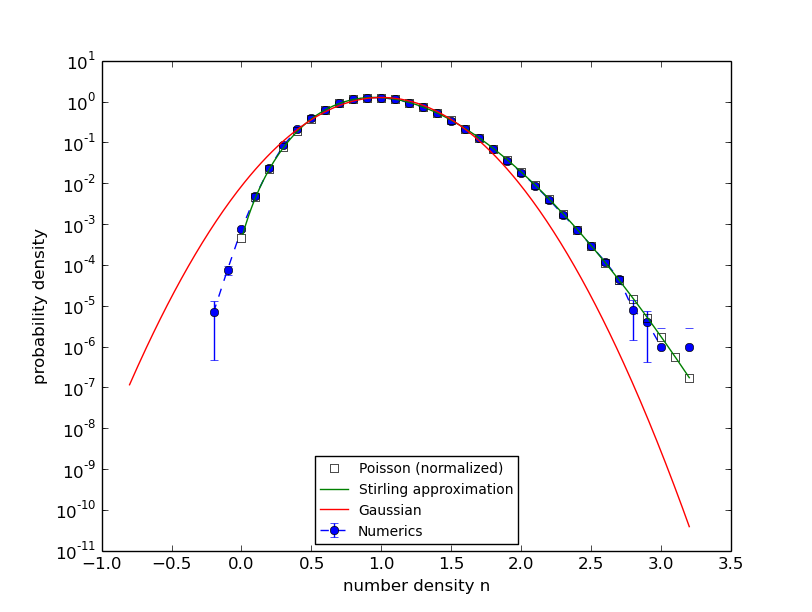
\includegraphics[width=0.5\linewidth]{fig1/1d_REACT_dt0.5_hist.png} &
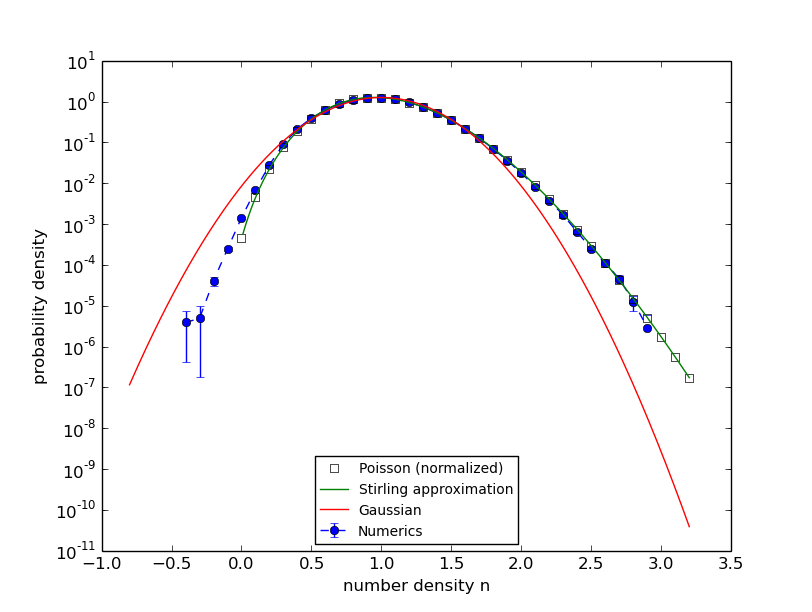
\includegraphics[width=0.5\linewidth]{fig1/1d_REACT_dt1_hist.png} \\ 
(e) $\Delta t=2$ & \\
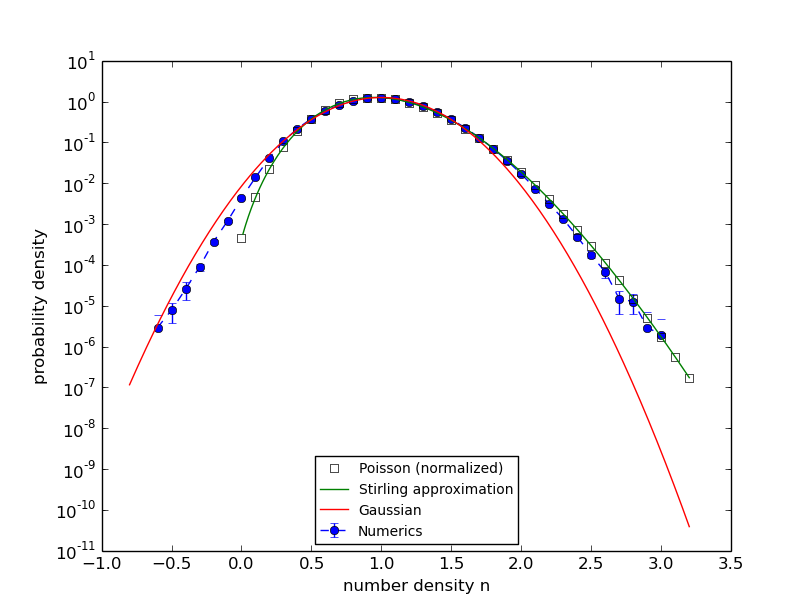
\includegraphics[width=0.5\linewidth]{fig1/1d_REACT_dt2_hist.png} &
\end{tabular}
\caption{\label{fig_1d_REACT_hist}}
\end{figure}


\begin{figure}
\begin{center}
\framebox[1.2\width]{2D, Diffusion-Only}
\end{center}
\begin{tabular}{cc}
(a) $\Delta t=0.1$ & (b) $\Delta t=0.25$ \\
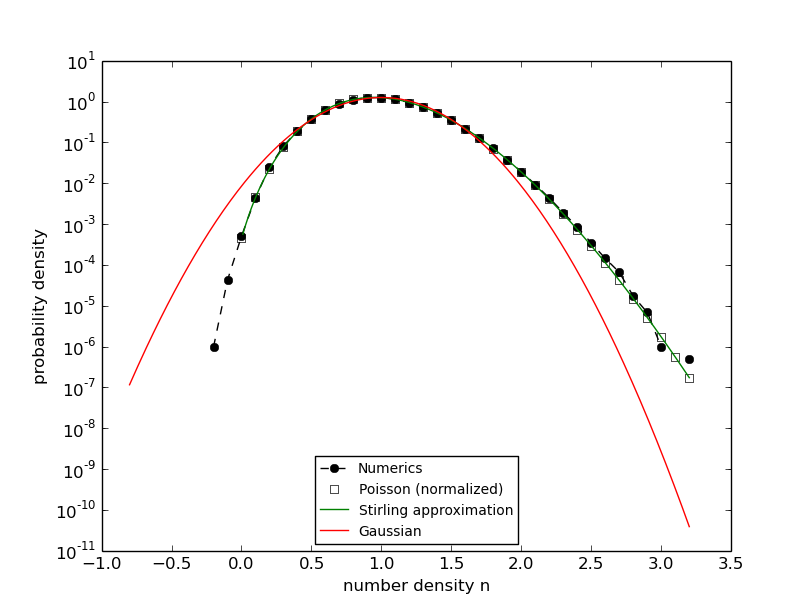
\includegraphics[width=0.5\linewidth]{fig1/2d_DIFF_dt0.1_hist.png} &
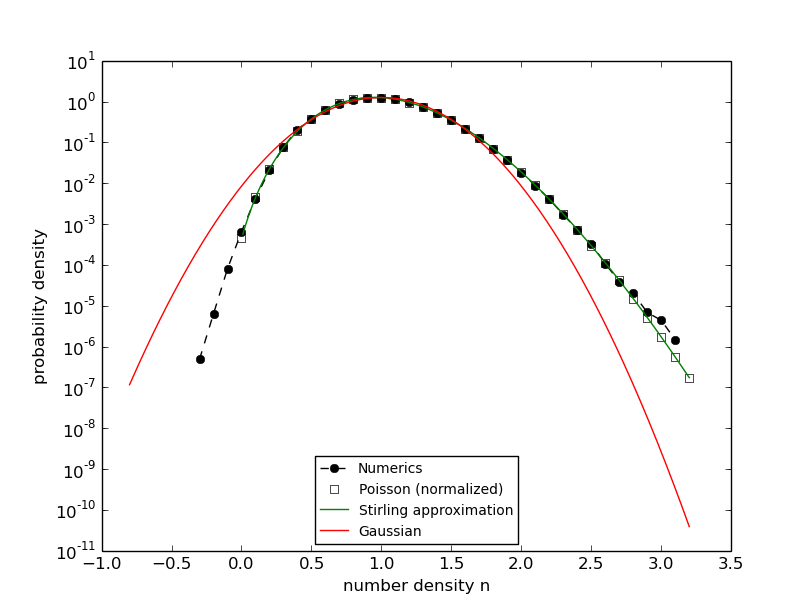
\includegraphics[width=0.5\linewidth]{fig1/2d_DIFF_dt0.25_hist.png} \\
(c) $\Delta t=0.5$ & (d) $\Delta t=1$ \\
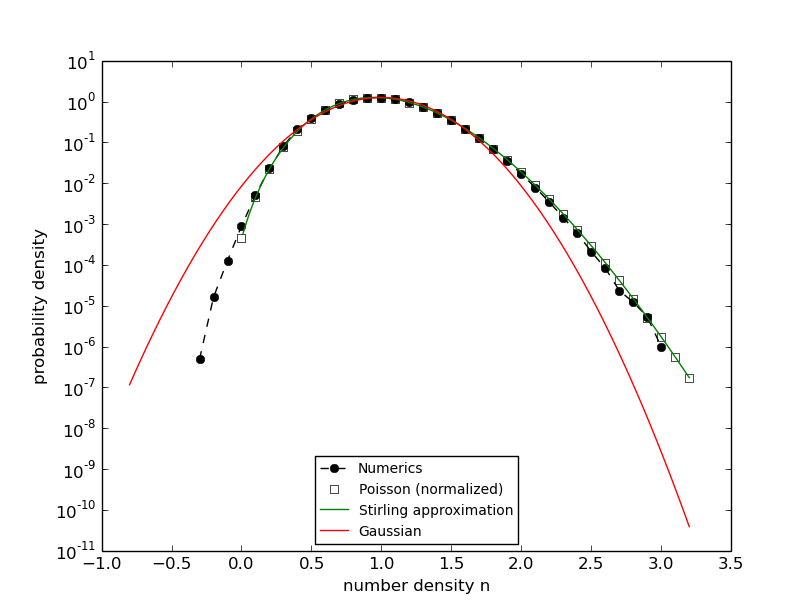
\includegraphics[width=0.5\linewidth]{fig1/2d_DIFF_dt0.5_hist.png} &
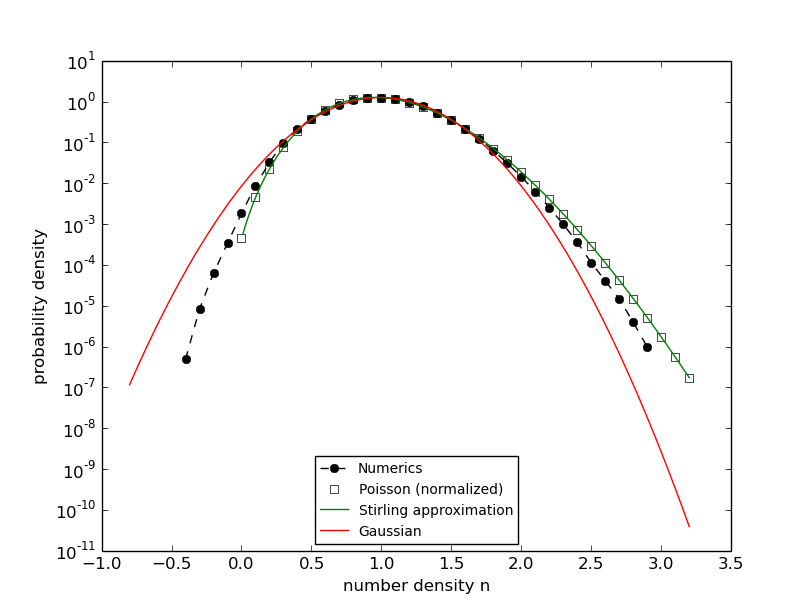
\includegraphics[width=0.5\linewidth]{fig1/2d_DIFF_dt1_hist.png} \\ 
(e) $\Delta t=2$ & \\
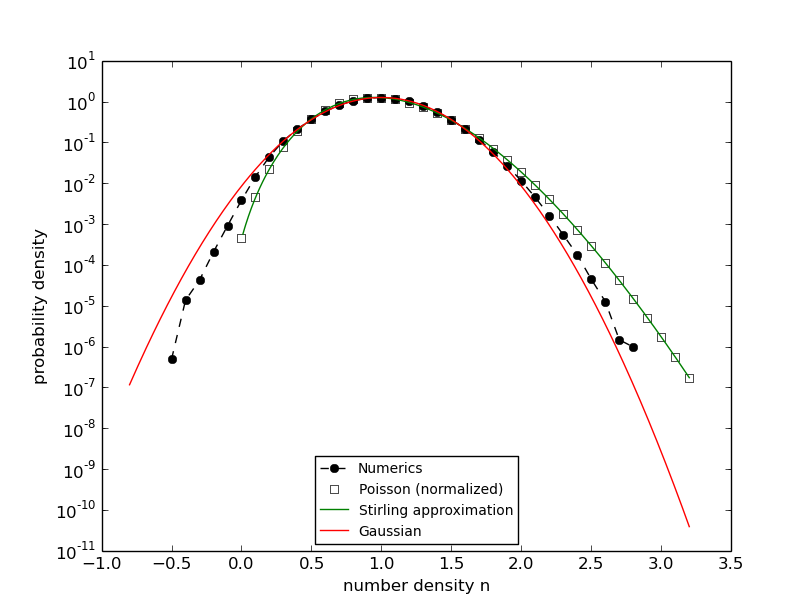
\includegraphics[width=0.5\linewidth]{fig1/2d_DIFF_dt2_hist.png} &
\end{tabular}
\caption{\label{fig_2d_DIFF_hist}}
\end{figure}

\begin{figure}
\begin{center}
\framebox[1.2\width]{2D, Reaction + Diffusion}
\end{center}
\begin{tabular}{cc}
(a) $\Delta t=0.1$ & (b) $\Delta t=0.25$ \\
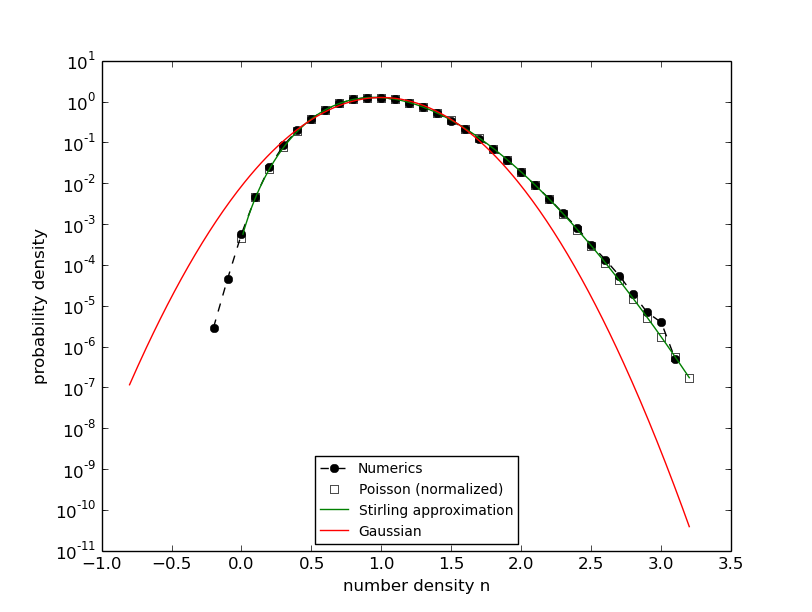
\includegraphics[width=0.5\linewidth]{fig1/2d_REACT_dt0.1_hist.png} &
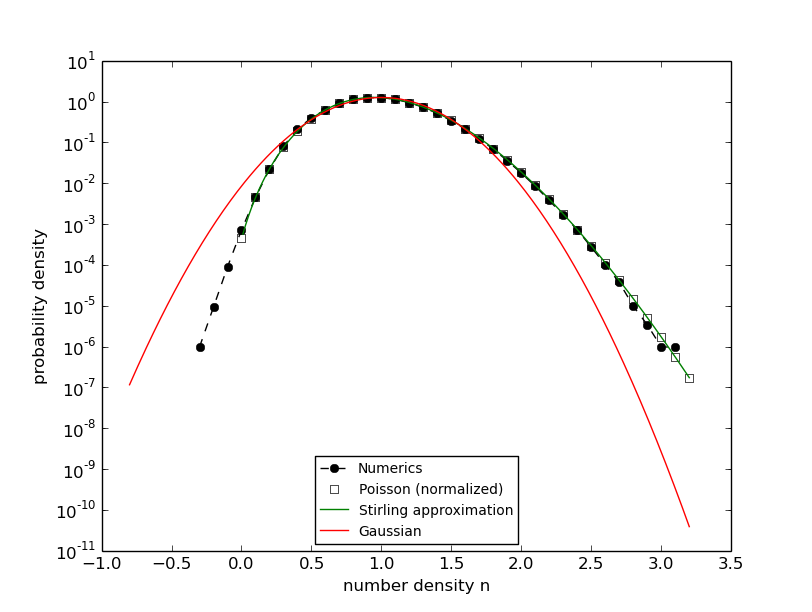
\includegraphics[width=0.5\linewidth]{fig1/2d_REACT_dt0.25_hist.png} \\
(c) $\Delta t=0.5$ & (d) $\Delta t=1$ \\
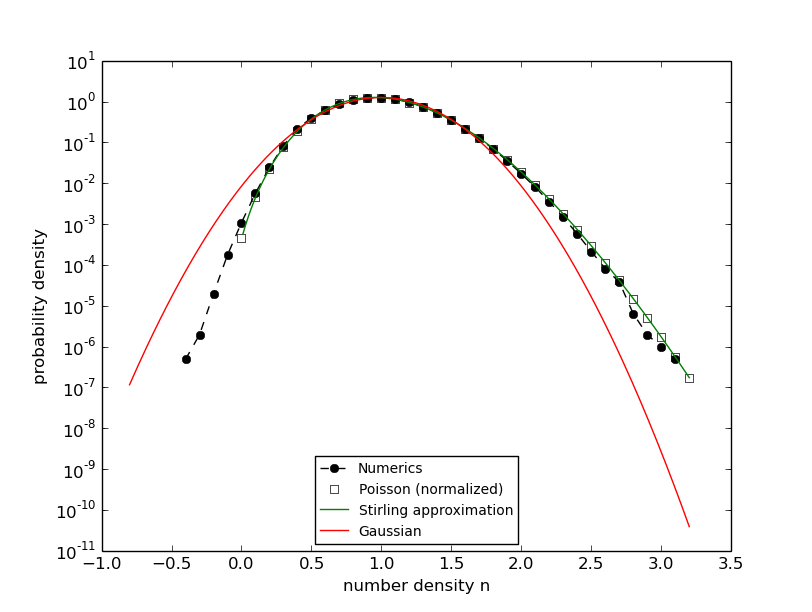
\includegraphics[width=0.5\linewidth]{fig1/2d_REACT_dt0.5_hist.png} &
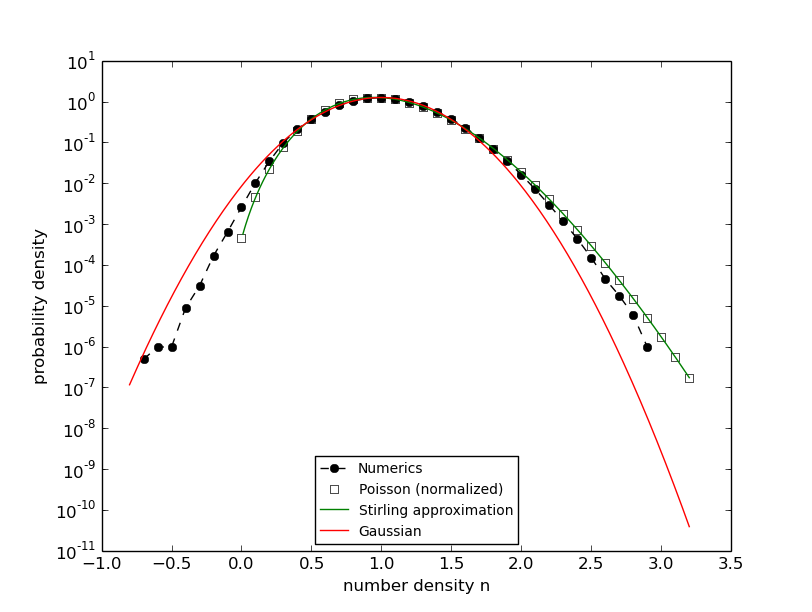
\includegraphics[width=0.5\linewidth]{fig1/2d_REACT_dt1_hist.png} \\ 
(e) $\Delta t=2$ & \\
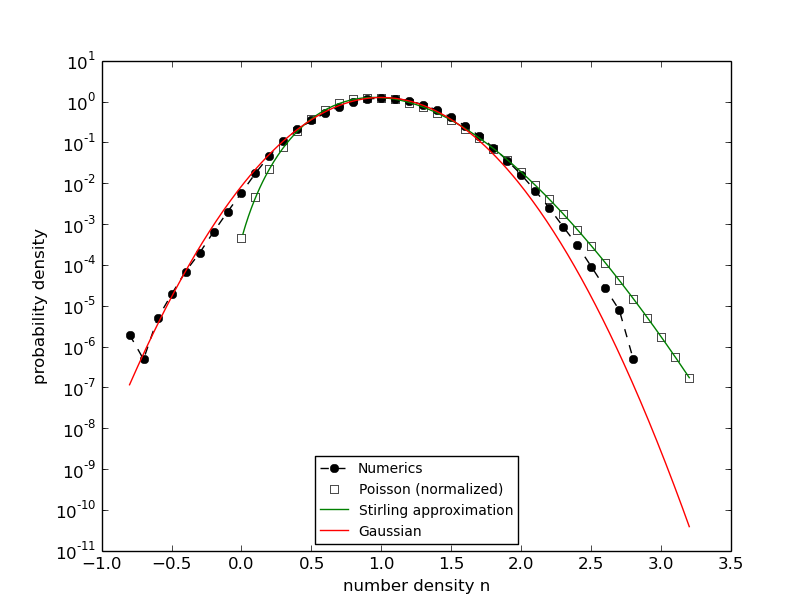
\includegraphics[width=0.5\linewidth]{fig1/2d_REACT_dt2_hist.png} &
\end{tabular}
\caption{\label{fig_2d_REACT_hist}}
\end{figure}


\begin{figure}
\begin{center}
\framebox[1.2\width]{3D, Diffusion-Only}
\end{center}
\begin{tabular}{cc}
(a) $\Delta t=0.1$ & (b) $\Delta t=0.25$ \\
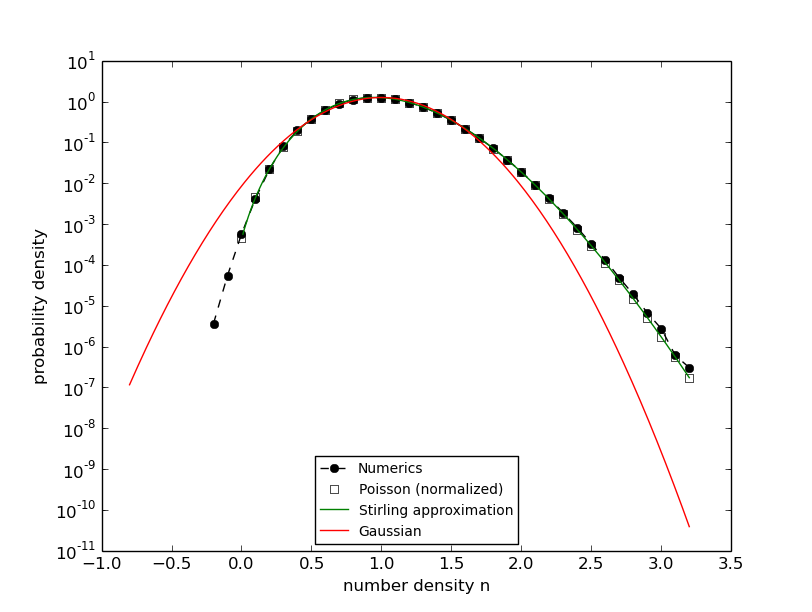
\includegraphics[width=0.5\linewidth]{fig1/3d_DIFF_dt0.1_hist.png} &
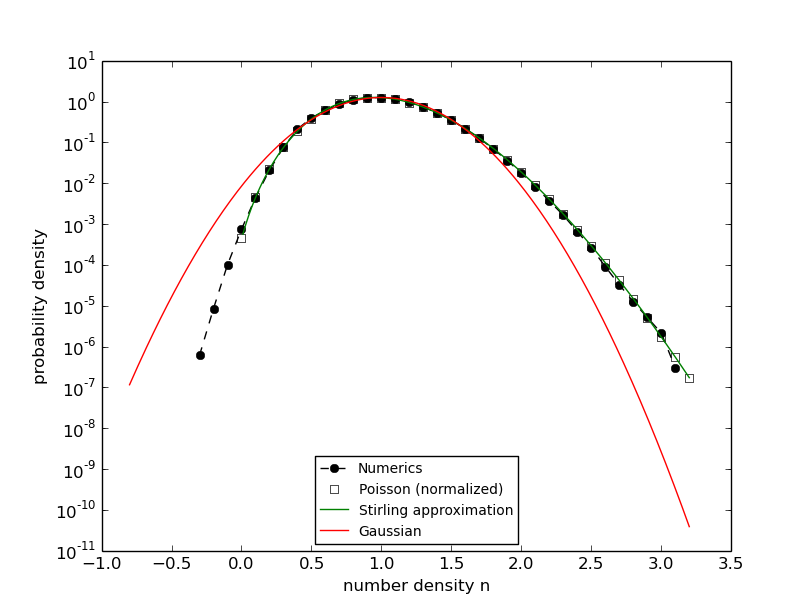
\includegraphics[width=0.5\linewidth]{fig1/3d_DIFF_dt0.25_hist.png} \\
(c) $\Delta t=0.5$ & (d) $\Delta t=1$ \\
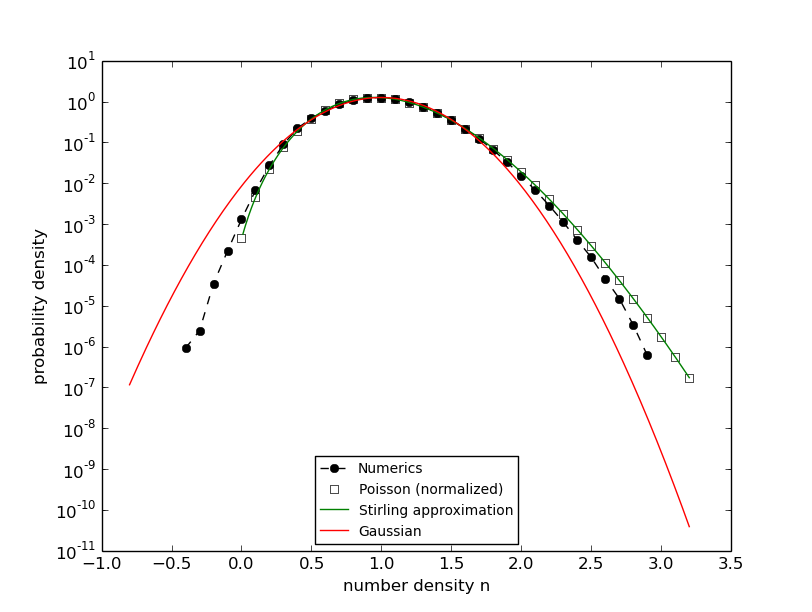
\includegraphics[width=0.5\linewidth]{fig1/3d_DIFF_dt0.5_hist.png} &
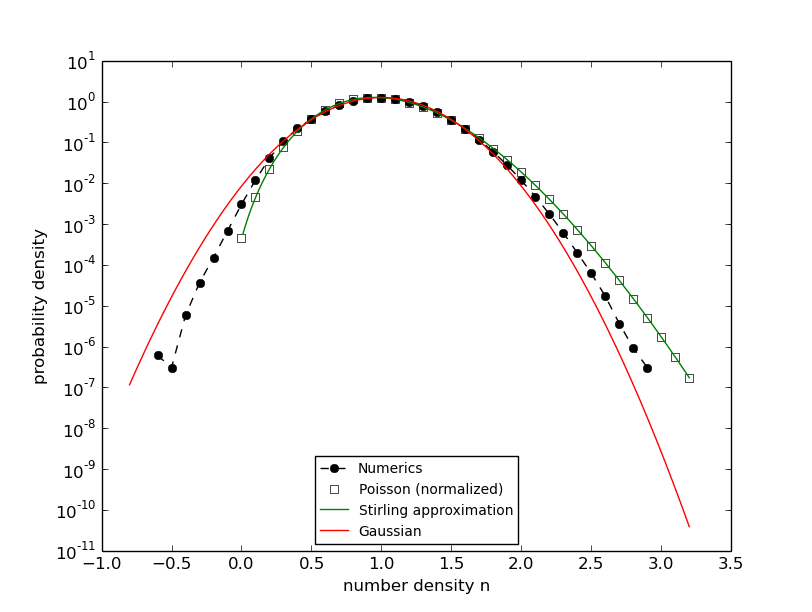
\includegraphics[width=0.5\linewidth]{fig1/3d_DIFF_dt1_hist.png} \\ 
(e) $\Delta t=2$ & \\
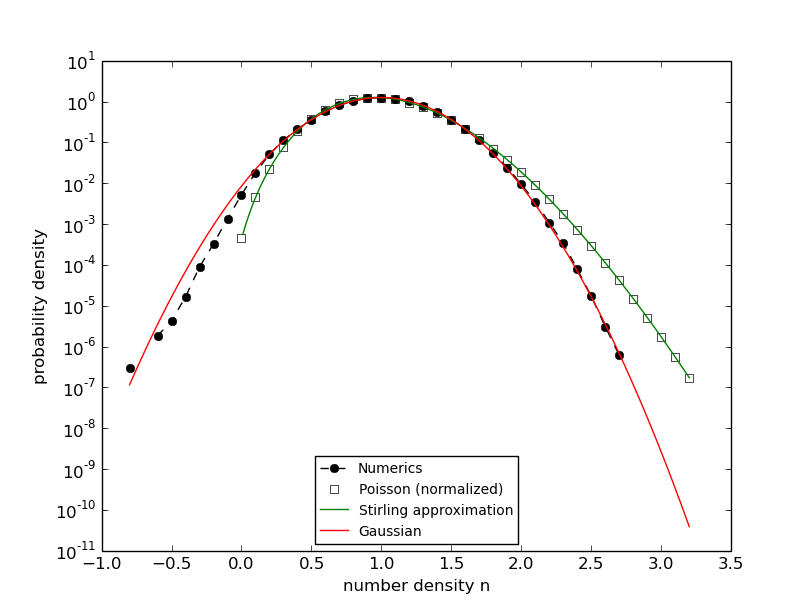
\includegraphics[width=0.5\linewidth]{fig1/3d_DIFF_dt2_hist.png} &
\end{tabular}
\caption{\label{fig_3d_DIFF_hist}}
\end{figure}

\begin{figure}
\begin{center}
\framebox[1.2\width]{3D, Reaction + Diffusion}
\end{center}
\begin{tabular}{cc}
(a) $\Delta t=0.1$ & (b) $\Delta t=0.25$ \\
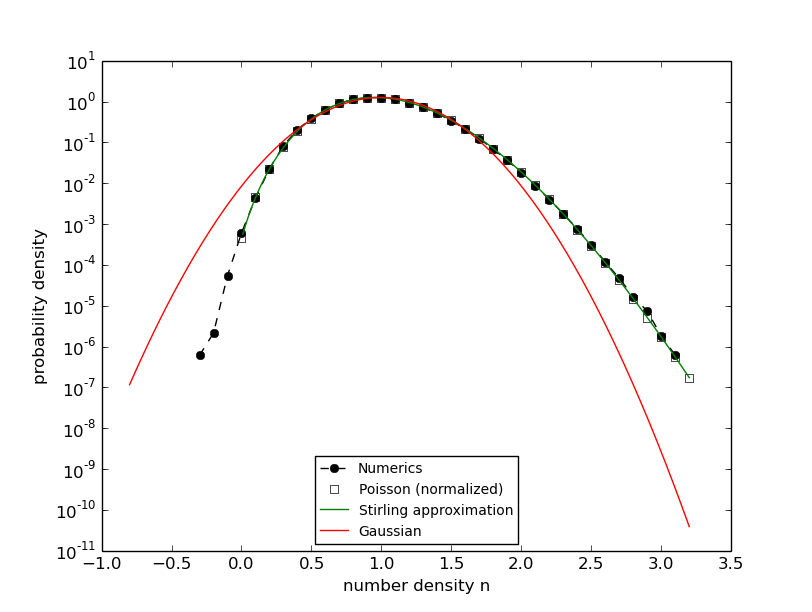
\includegraphics[width=0.5\linewidth]{fig1/3d_REACT_dt0.1_hist.png} &
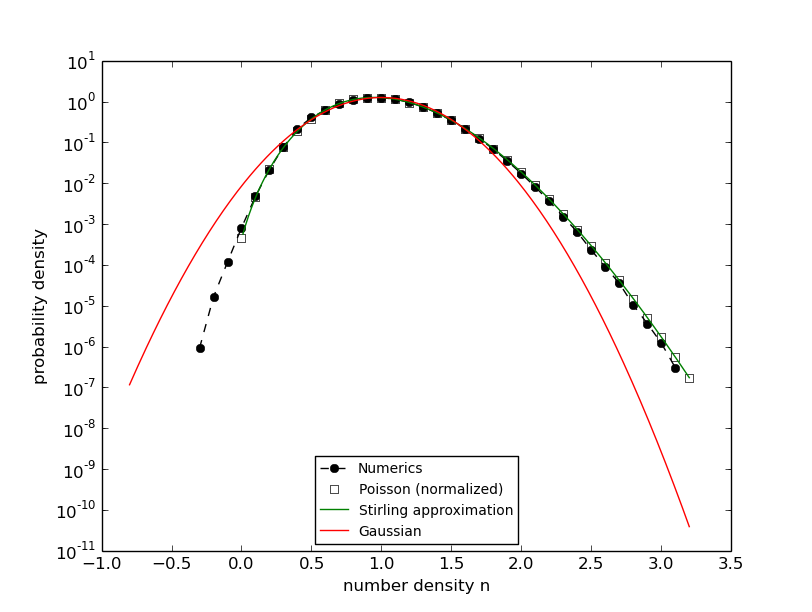
\includegraphics[width=0.5\linewidth]{fig1/3d_REACT_dt0.25_hist.png} \\
(c) $\Delta t=0.5$ & (d) $\Delta t=1$ \\
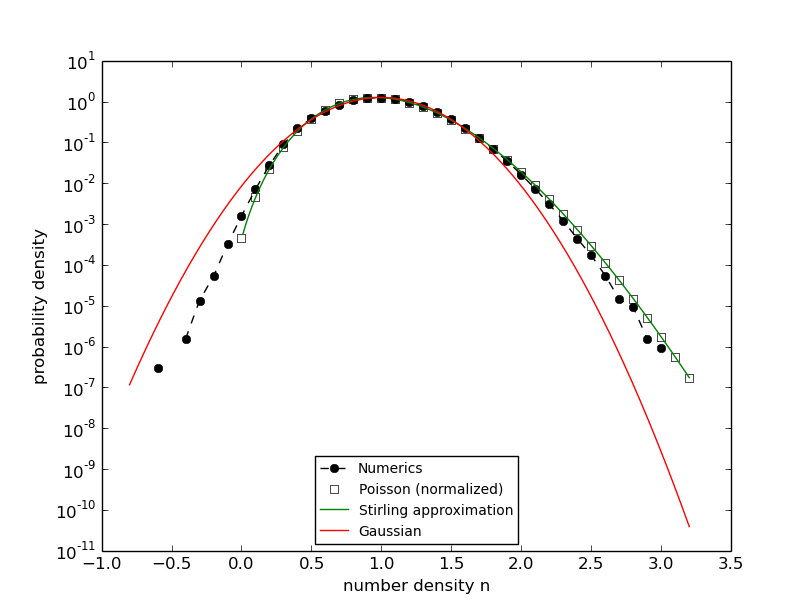
\includegraphics[width=0.5\linewidth]{fig1/3d_REACT_dt0.5_hist.png} &
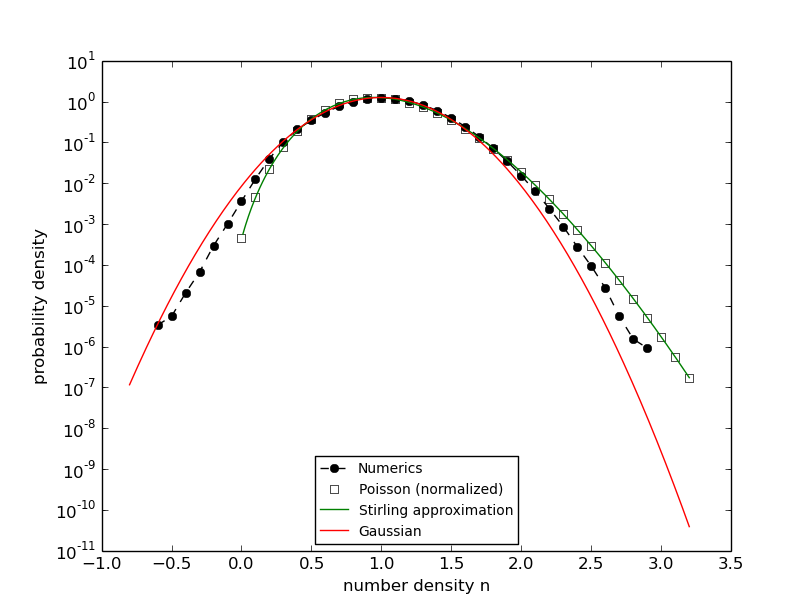
\includegraphics[width=0.5\linewidth]{fig1/3d_REACT_dt1_hist.png} \\ 
(e) $\Delta t=2$ & \\
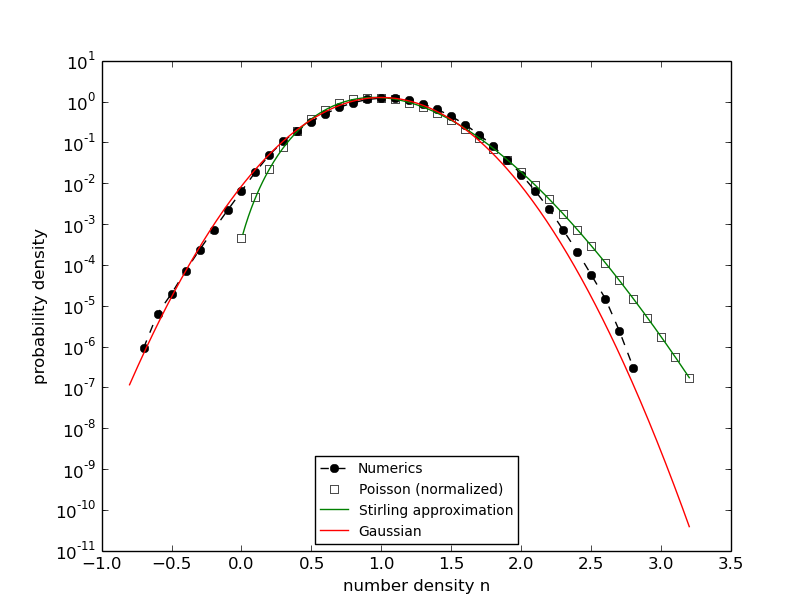
\includegraphics[width=0.5\linewidth]{fig1/3d_REACT_dt2_hist.png} &
\end{tabular}
\caption{\label{fig_3d_REACT_hist}}
\end{figure}

\end{document}
